\begin{frame}{patch instruction?}
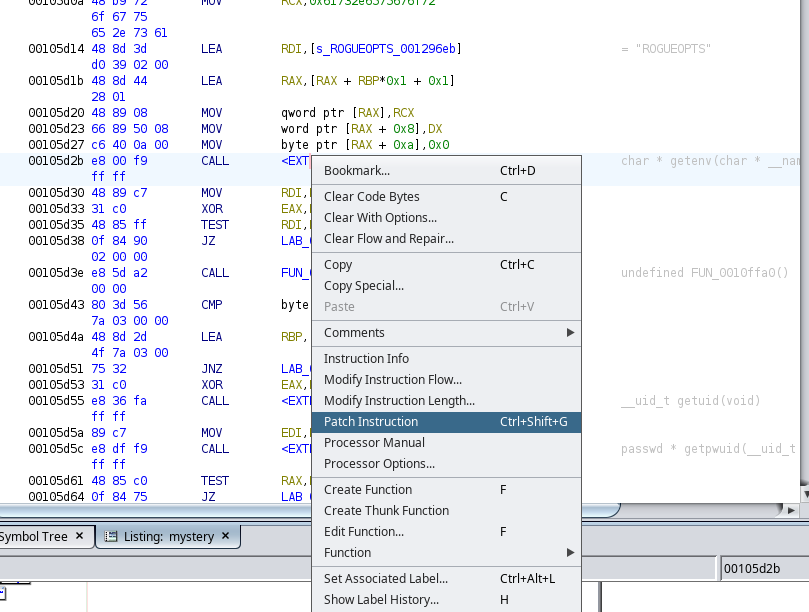
\includegraphics[width=\textwidth]{../re-tools/ghidra-patch-ex}
\end{frame}

\begin{frame}{patch instruction?}
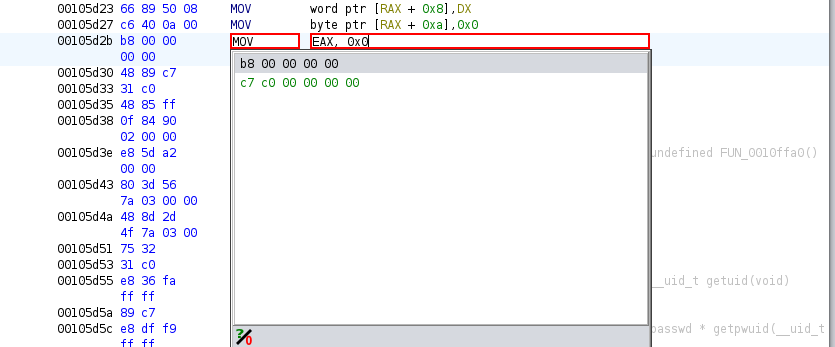
\includegraphics[width=\textwidth]{../re-tools/ghidra-patch-ex2}
\end{frame}

\begin{frame}{why is this useful?}
    \begin{itemize}
    \item can export modified version of binary to test
    \item ghidra has support for debugging or emulating running program
        \begin{itemize}
        \item emulation is another application of PCode representation
        \item debugging requires some work to configure
        \end{itemize}
    \end{itemize}
\end{frame}

